\newcommand{\figoverview}{
\begin{figure}[tbp]
\begin{center}
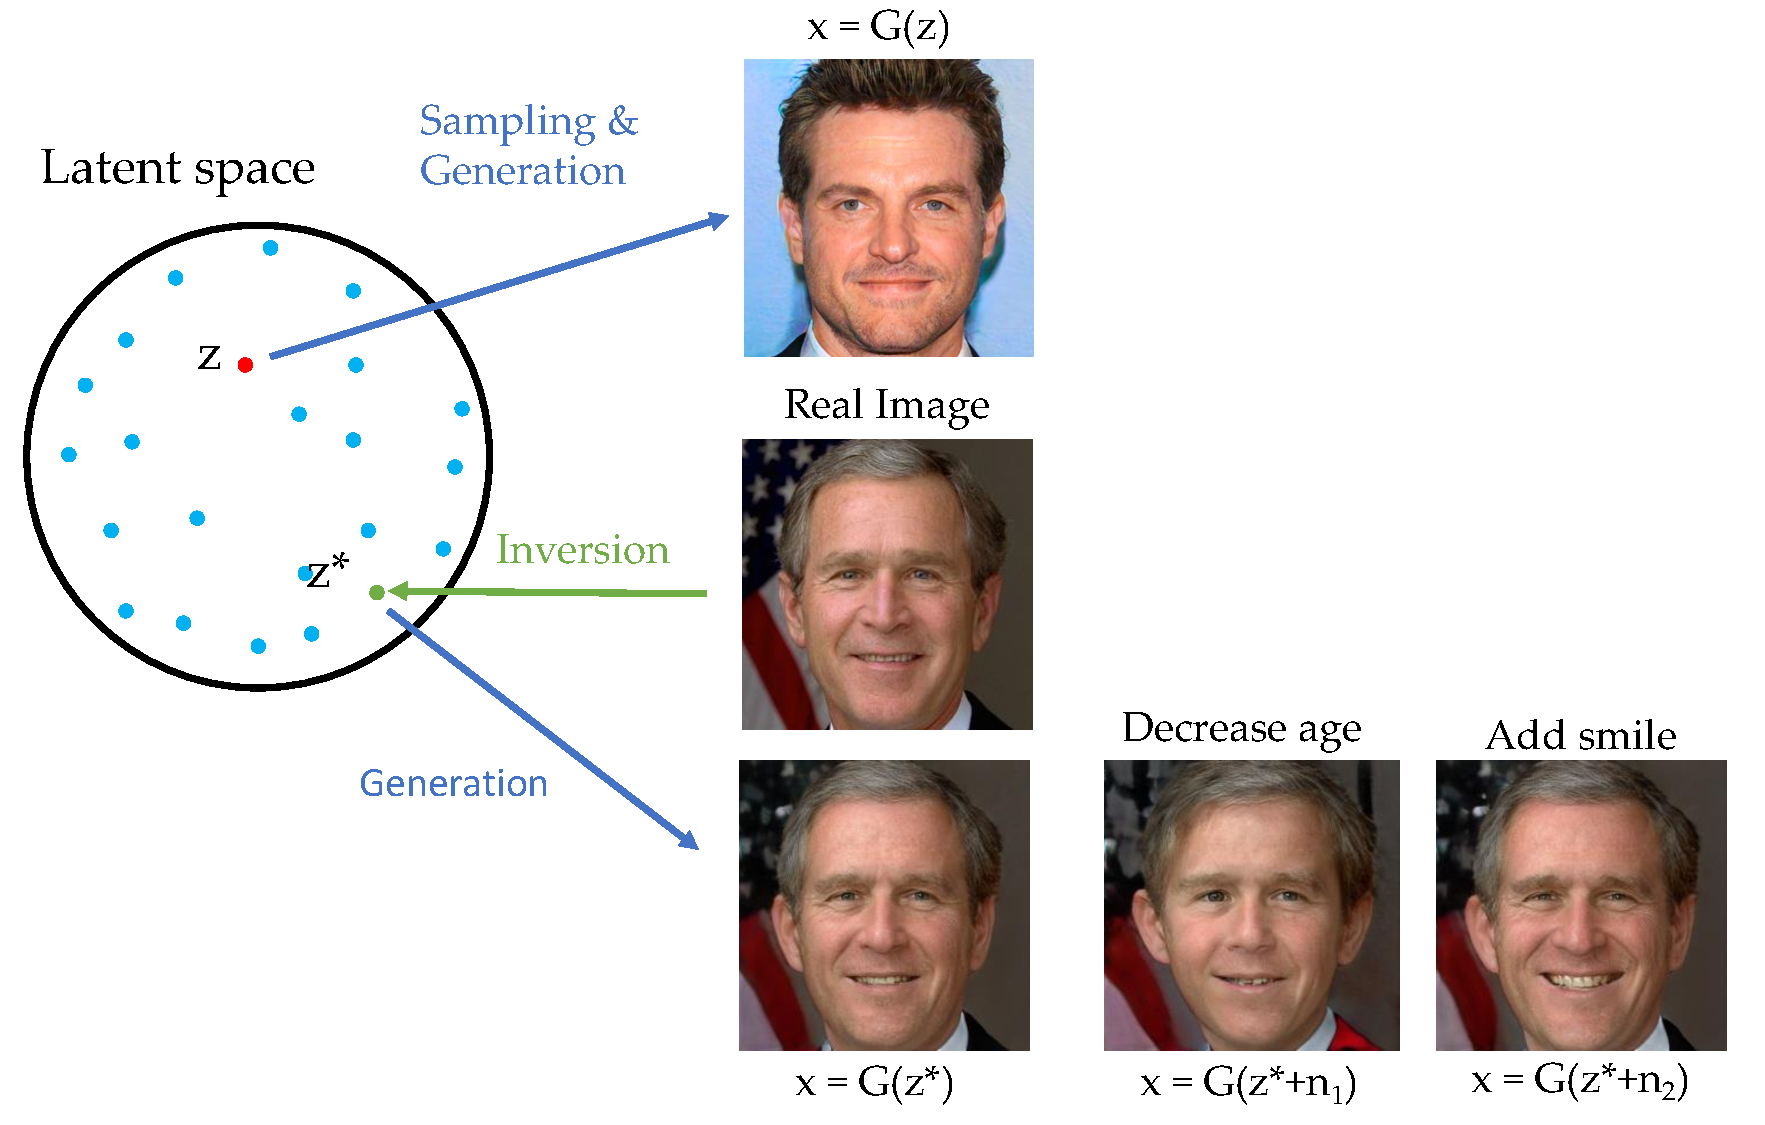
\includegraphics[width=0.9\linewidth]{images/overview_zhou}
\end{center}
\caption{\textbf{Illustration of GAN inversion.} Different from the conventional sampling and generation process using trained generator $G$, GAN inversion maps a given real image $x$ to the latent space and obtains the latent code $\mathbf{z^{*}}$. The reconstructed image $x^{*}$ is then obtained by $x^*=G(\mathbf{z^{*}})$. By varying the latent code $\mathbf{z^{*}}$ in different interpretable directions \eg, $\mathbf{z^{*}}+\mathbf{n_1}$ and $\mathbf{z^{*}}+\mathbf{n_2}$ where $\mathbf{n_1}$ and $\mathbf{n_2}$ model the age and smile in the latent space respectively, we can edit the corresponding attribute of the real image. The reconstructed results are from \cite{zhu2020indomain}.
}
\label{fig:overview}
\end{figure}
}

\newcommand{\figtype}{
\begin{figure}[tbp]
\begin{center}
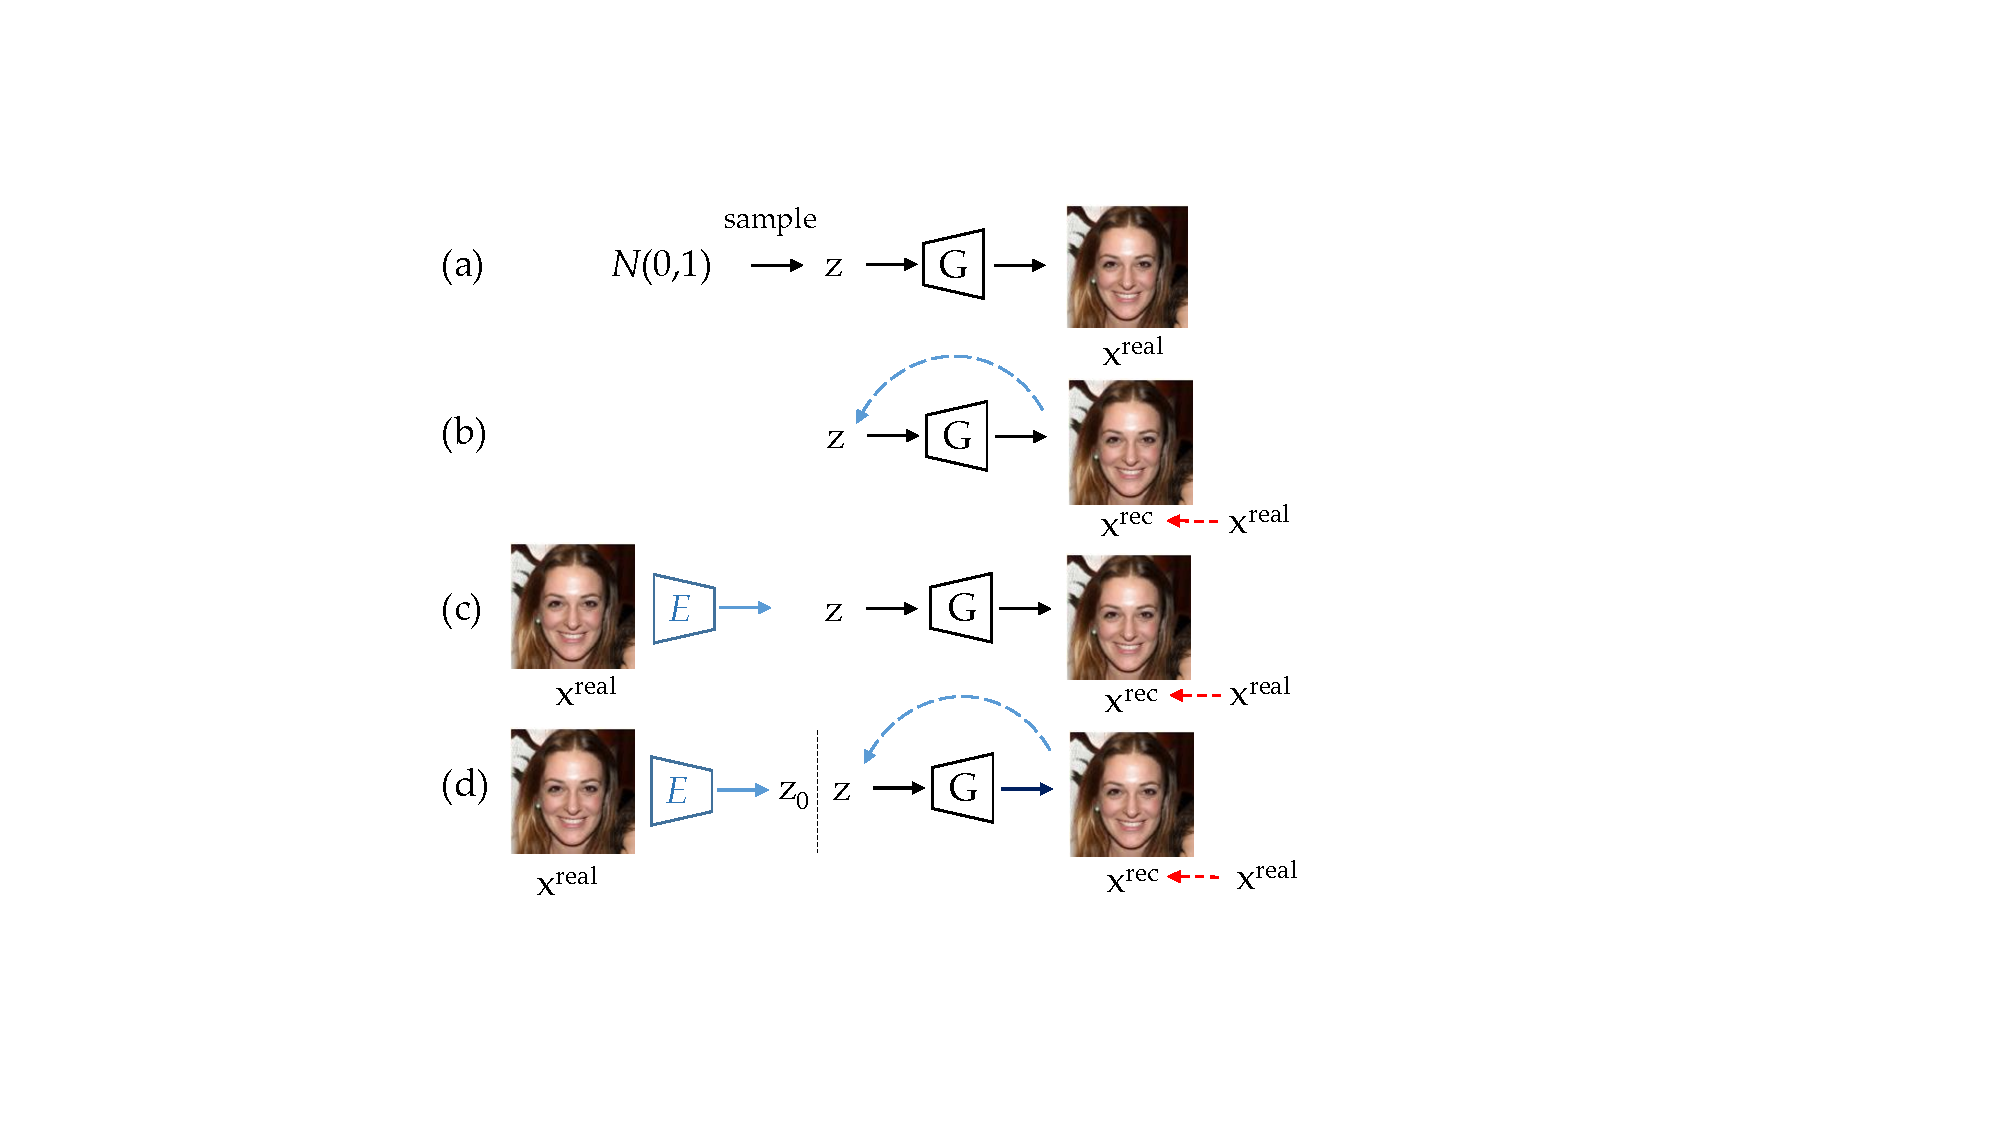
\includegraphics[width=0.95\linewidth]{images/inversion_types}
\end{center}
\caption{\textbf{Illustration of GAN Inversion Methods.} 
(a) given a well-trained GAN model, photo-realistic images can be generated from randomly sampled latent vectors. 
(b) {\bf optimization-based} inversion uses an optimization algorithm to iteratively optimize the latent code to minimize the pixel-wise reconstruction loss. 
(c) {\bf learning-based} inversion builds an encoder network that maps an image into the latent space. 
(d) {\bf hybrid} approach uses the encoder to generate an initialization for optimization, \ie, an encoder network is first used to obtain an approximate embedding and then refine it with an optimization algorithm.}
\label{fig:inversion_types}
\end{figure}
}

\newcommand{\figwalk}{
\begin{figure}[t]
\centering
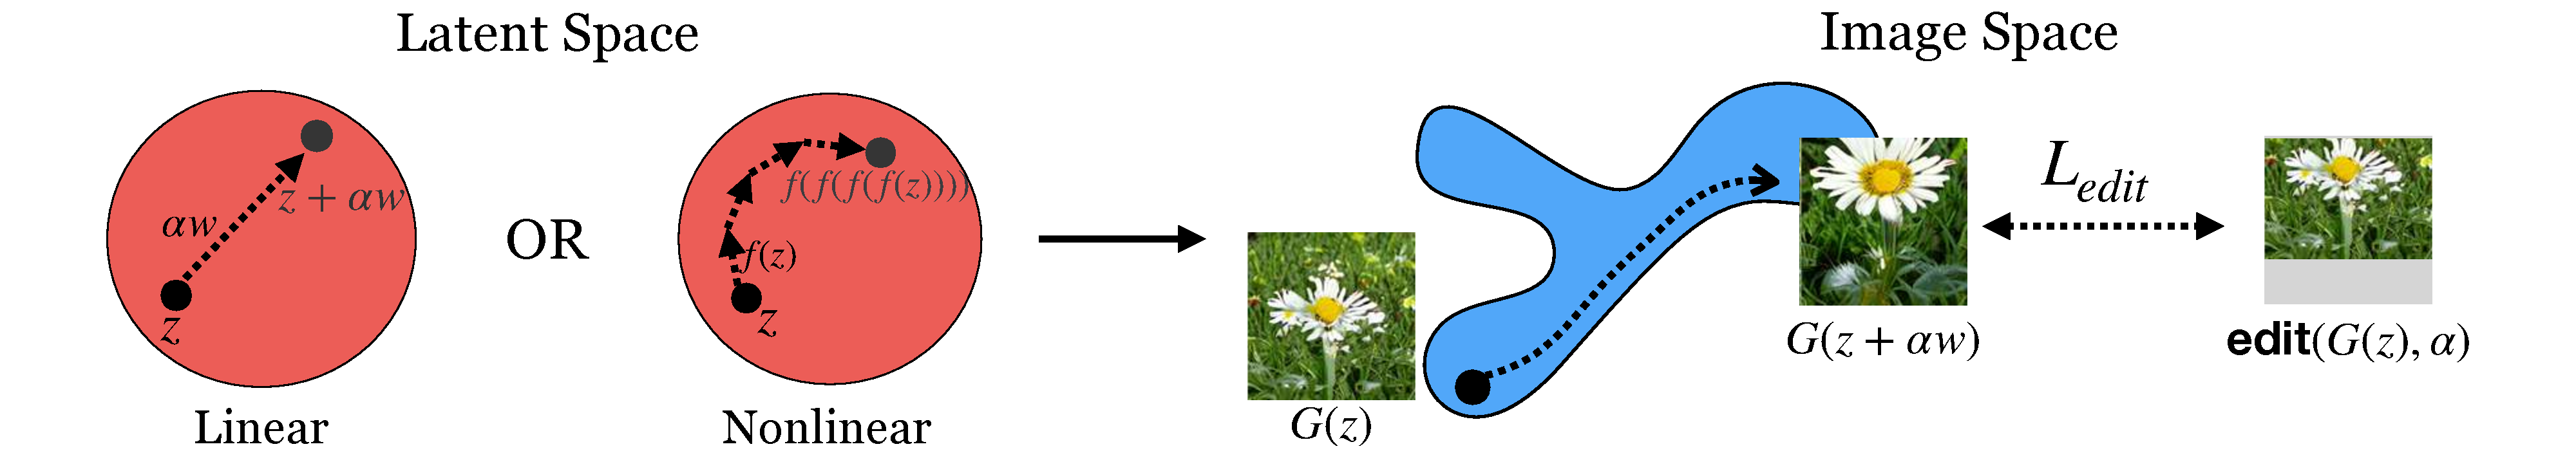
\includegraphics[width=1\columnwidth]{images/walk.pdf}
\caption{Illustration of discovering interpretable directions in the latent space~\cite{jahanian2020steerability}. 
The goal is to find a path in $\mathcal{Z}$ space to transform the generated image $G(\mathbf{z})$ to its edited version $\texttt{edit}(G(\mathbf{z},\alpha))$, \eg, an $\alpha \times$ zoom. 
The transformation can be represented as $G(\mathbf{z}+\alpha \mathbf{w})$ for a linear walk or $G(f(f(...(\mathbf{z})))$ for a non-linear walk.}
\label{fig:walk}
\end{figure}
}

\newcommand{\figindomain}{
\begin{figure}[tbp]
\begin{center}
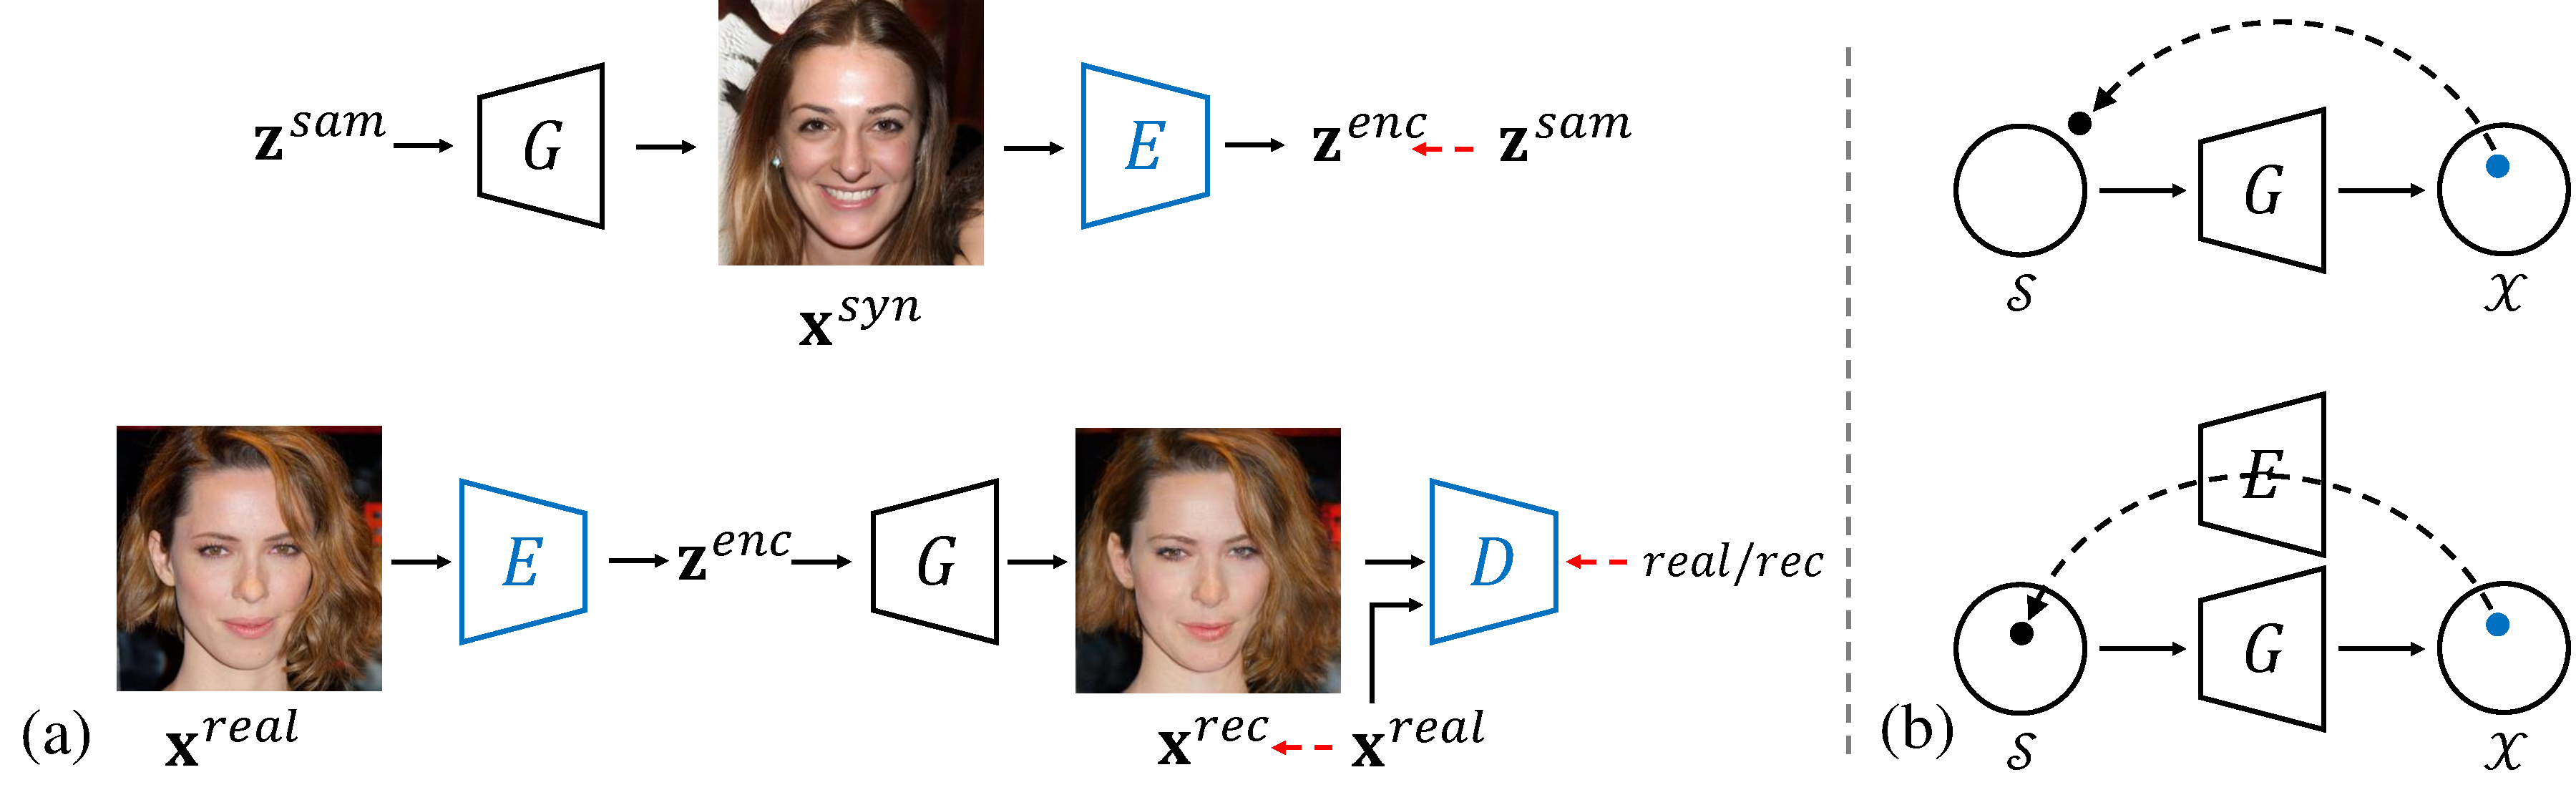
\includegraphics[width=0.95\linewidth]{images/indomain_comp.pdf}
\end{center}
\caption{\textbf{Comparisons between the training of (upper) conventional encoder and (lower) domain-guided encoder proposed in~\cite{zhu2020indomain} for GAN inversion.} Blue blocks represent trainable models and red dashed arrows indicate the supervisions. The domain-guided encoder is trained to recover the real images, instead of being trained with synthesized data to recover the latent code. The generator $G$ is well-trained with fixed weights during training $E$. (b) The comparison between the conventional optimization and the domain-regularized optimization proposed in~\cite{zhu2020indomain}. The well-trained domain-guided encoder $E$ is involved as a regularization to fine-tune the latent code in the semantic domain during $\mathbf{z}$ optimization.}
\label{fig:indomain}
\end{figure}
}

\newcommand{\fignoninference}{
\begin{figure}[tbp]
\begin{center}
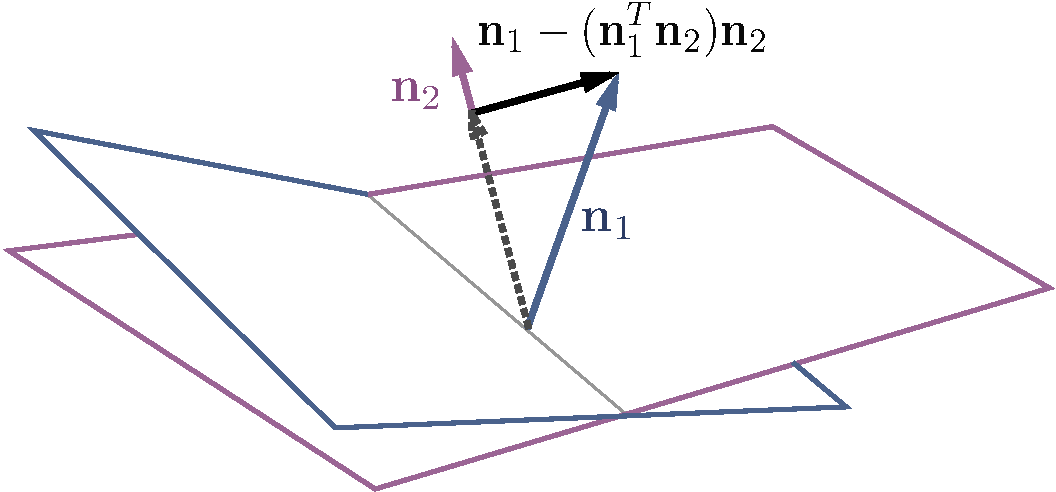
\includegraphics[width=0.6\linewidth]{images/projection}
\end{center}
\caption{\textbf{Illustration of the non-interference property in subspace.} The projection of $\mathbf{n}_{1}$ onto $\mathbf{n}_{2}$ is subtracted from $\mathbf{n}_{1},$ resulting in a new direction $\mathbf{n}_{1}-(\mathbf{n}_{1}^{\top} \mathbf{n}_{2}) \mathbf{n}_{2}$. This figure is from~\cite{shen2020interpreting}.}
\label{fig:projection}
\end{figure}
}

\newcommand{\figroi}{
\begin{figure}[tbp]
\centering
%\vspace{-0.5cm} 
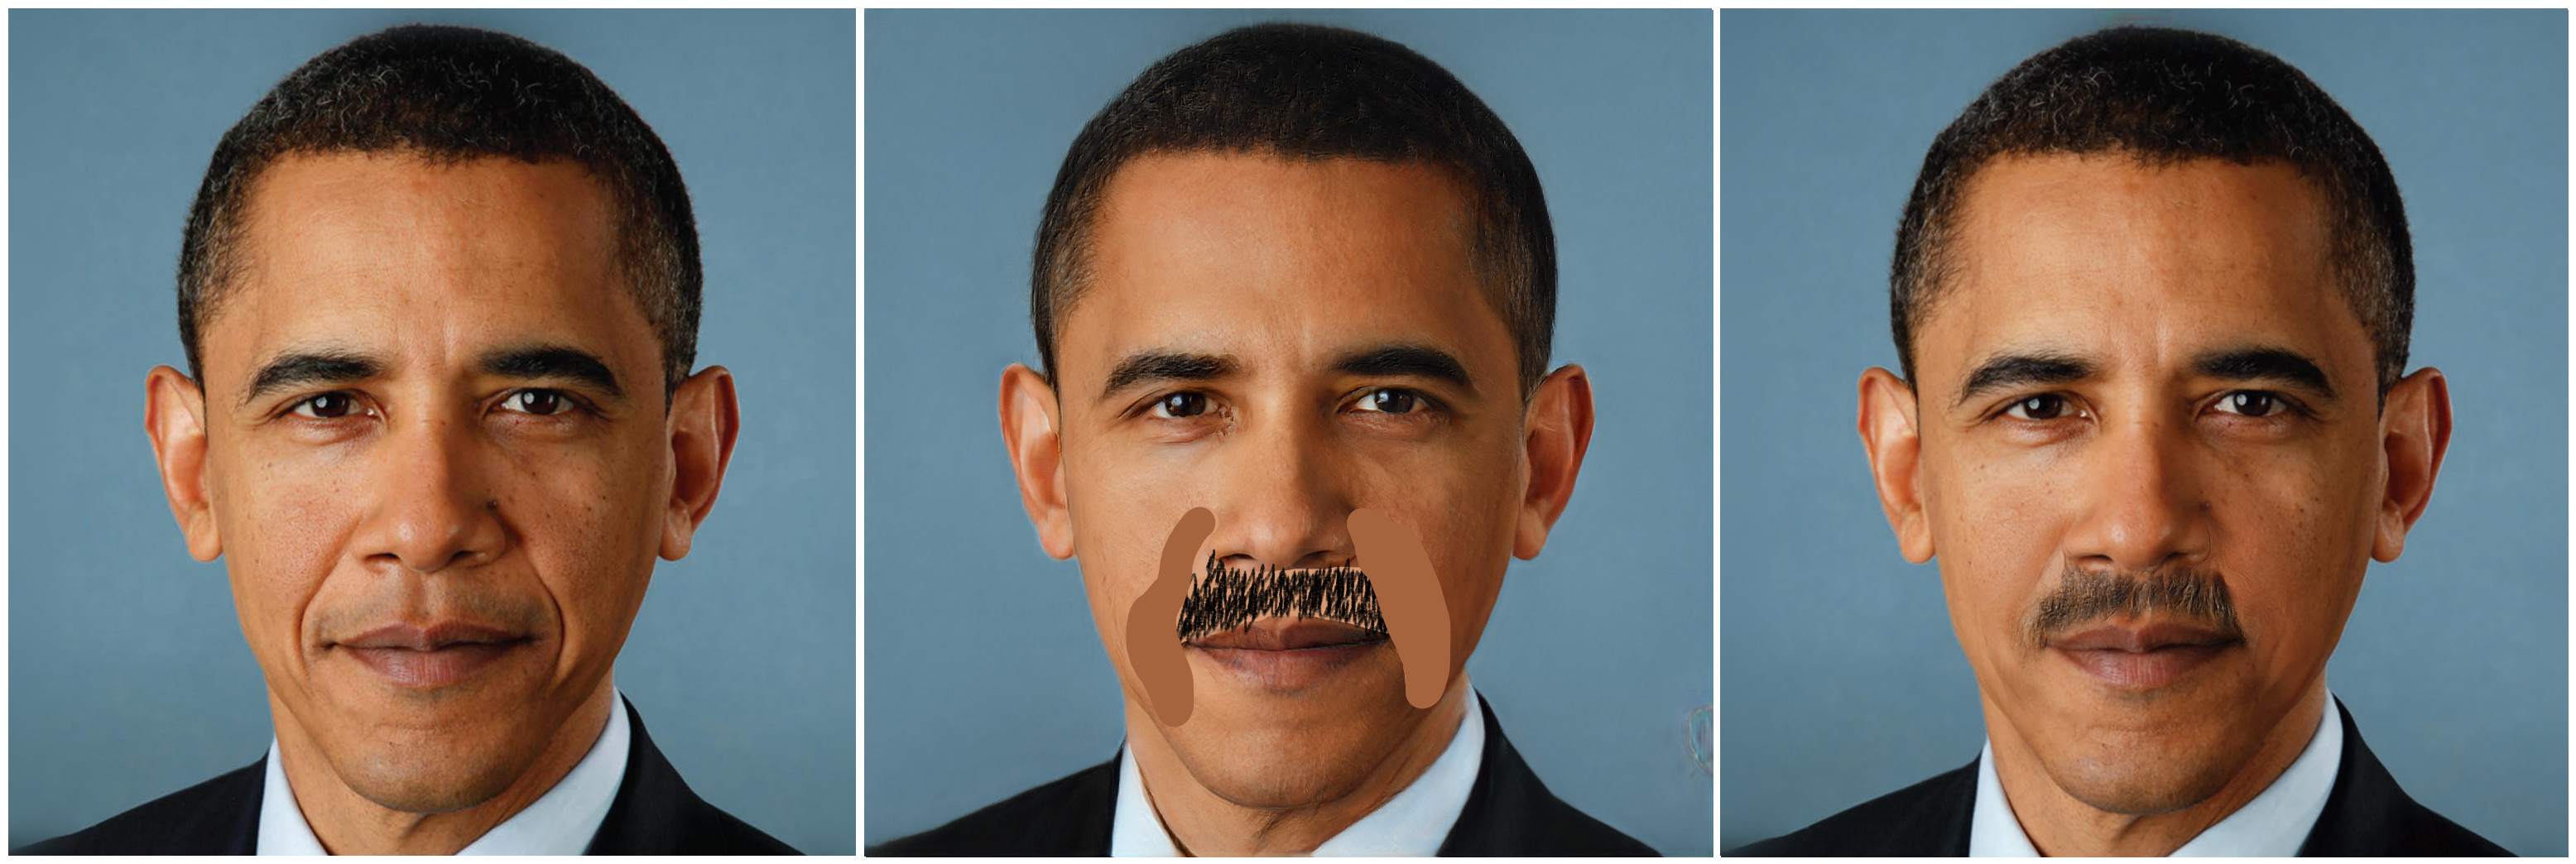
\includegraphics[width= 0.95\linewidth]{images/local_obama.jpg}
 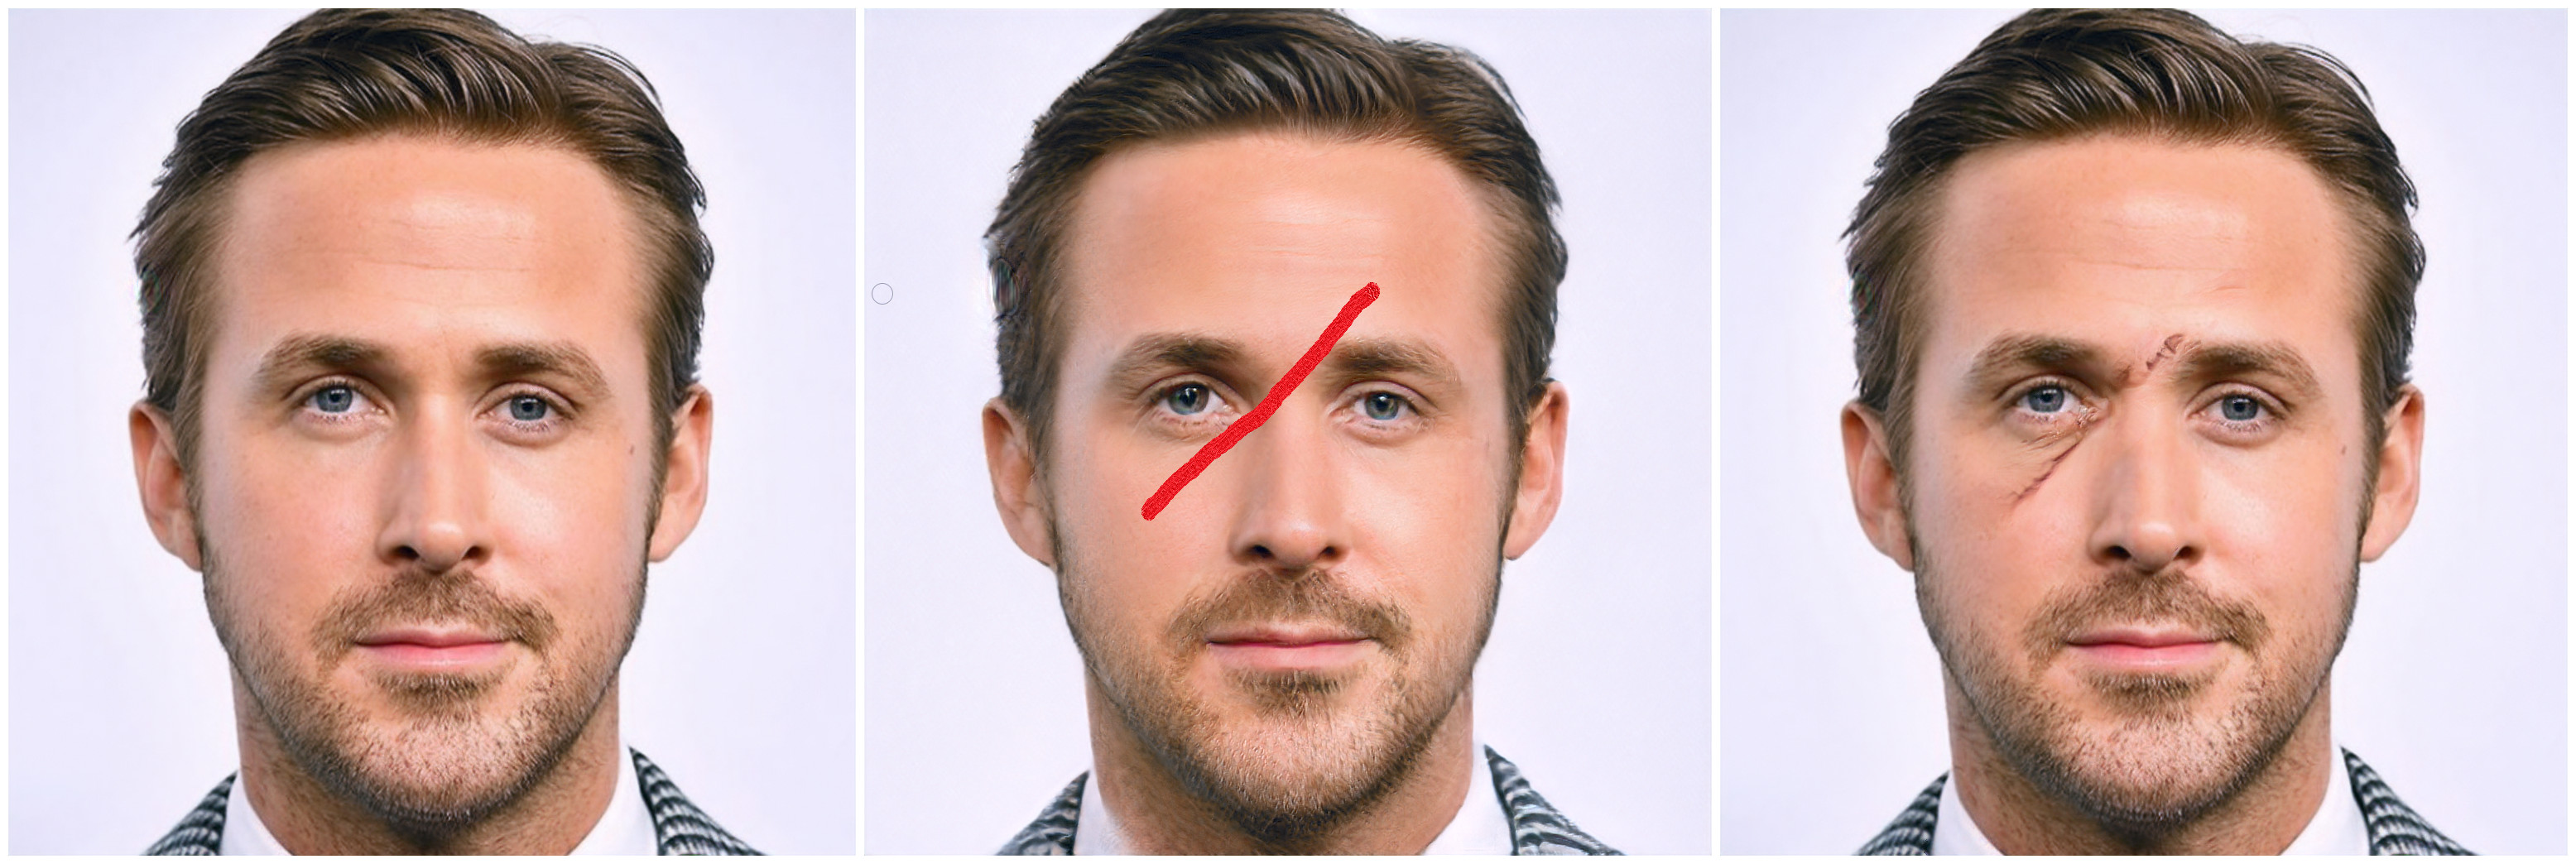
\includegraphics[width=0.95\linewidth]{images/local_ryan.jpg}
\caption{\textbf{Illustration of region-of-interest editing~\cite{abdal2020image2stylegan2}.} From left to right: base image; scribbled image; result of local edits.}
\label{fig:local}
\end{figure}
}

\newcommand{\figrewrite}{
\begin{figure}[tbp]
\begin{center}
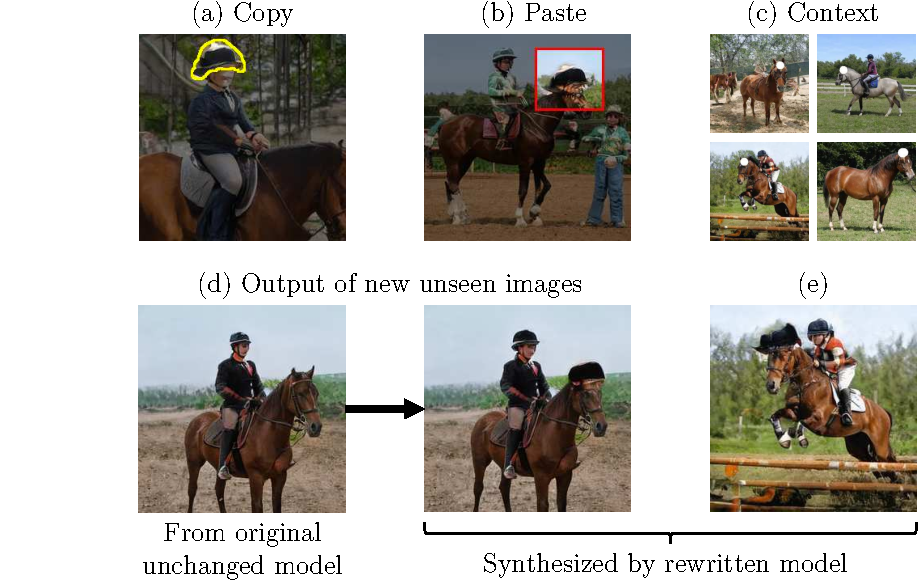
\includegraphics[width=0.95\linewidth]{images/ganrewriting}
\end{center}
\caption{\textbf{Copy-Paste-Context interface for rewriting a model~\cite{zhu2016generative}.} 
%The first row is the user inputs and the last are corresponding model outputs. 
(a) Copy: the user uses a brush to select a region containing an interesting object or shape, defining the target. (b) Paste: The user positions and pastes the copied object into a single target image. (c) Context: To control generalization, the user selects target regions in several images. (d) The edit is applied to the model, not to a specific image, such that newly generated images will have hats on top of horse heads. (e) The change has been applied to different types of horses and poses.}
\label{fig:ganrewriting}
\end{figure}
}

\newcommand{\figood}{
\begin{figure}[tbp]
\begin{center}
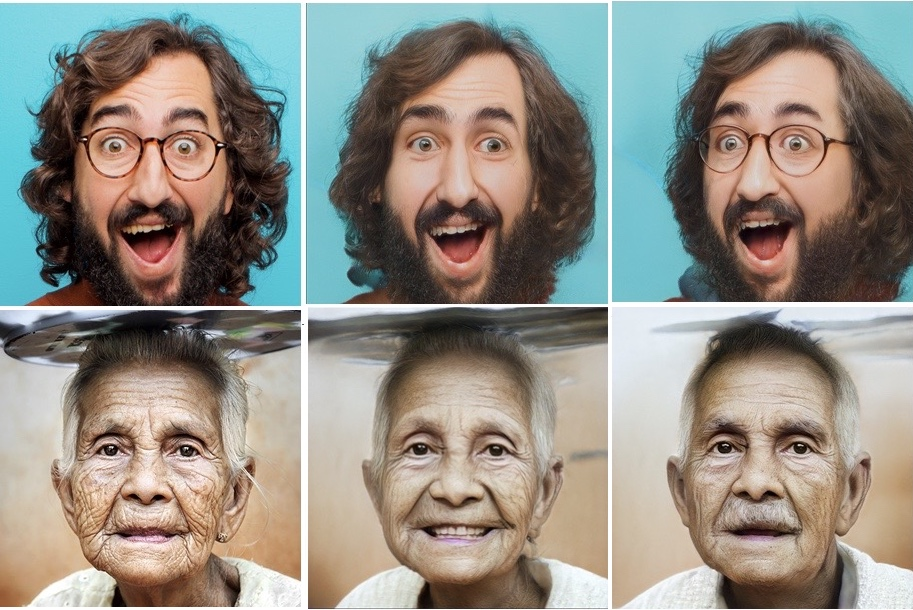
\includegraphics[width=0.95\linewidth]{images/ood}
\end{center}
\caption{\textbf{Illustration of face image manipulation.} These are real image editing results from using StyleFlow~\cite{abdal2020styleflow}.}
\label{fig:ood}
\end{figure}
}

\newcommand{\figapp}{
\begin{figure}[tbp]
\begin{center}
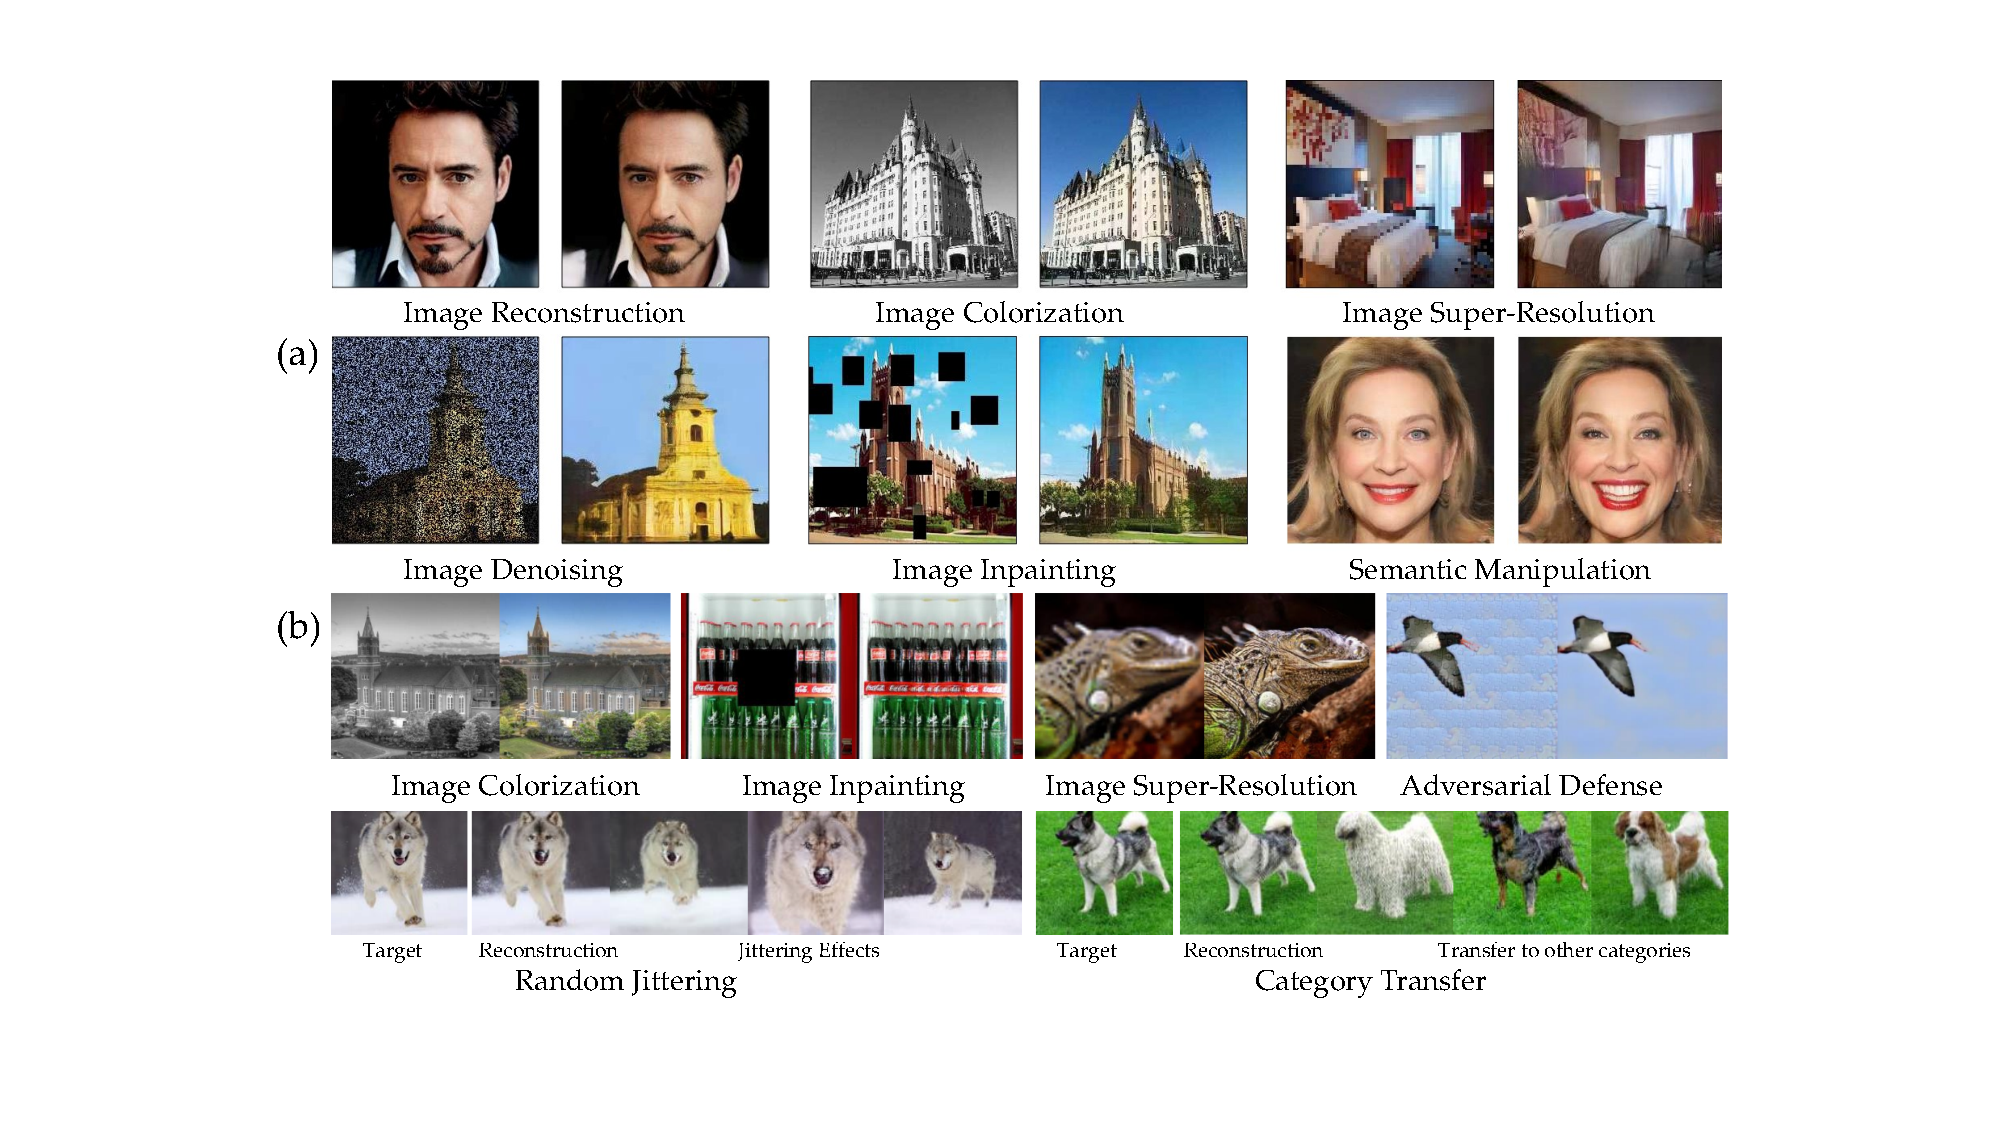
\includegraphics[width=0.95\linewidth]{images/application_zhou}
\end{center}
\caption{\textbf{Illustration of image processing using GAN inversion.}
GAN inversion does not require task-specific dense-labeled datasets and can be applied to many tasks like image reconstruction, image restoration and image manipulation. 
% GAN inversion does not require task-specific dense-labeled datasets and can be applied to many tasks like image reconstruction (a), image restoration (b)(c)(d)(e) and image manipulation (f). 
The upper illustration (a) is from mGANPrior~\cite{gu2020image} and the lower (b) is from DGP~\cite{pan2020exploiting}.}
\label{fig:application}
\end{figure}
}

\newcommand{\figcorrect}{
\begin{figure}[tbp]
\begin{center}
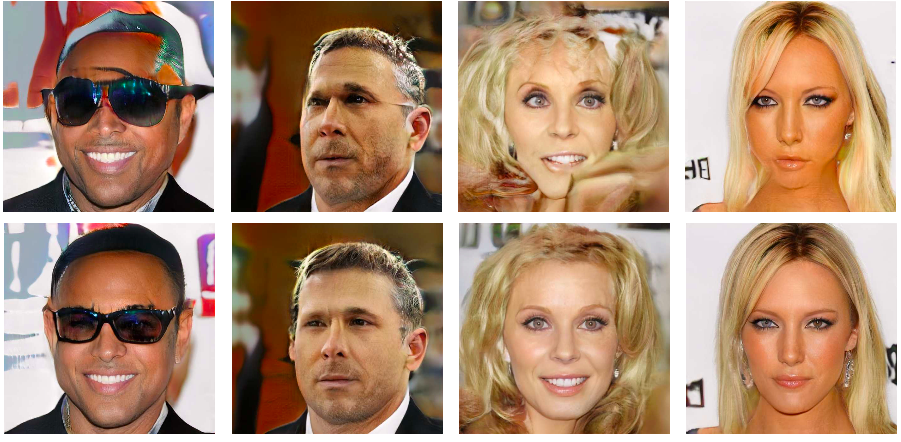
\includegraphics[width=0.98\linewidth]{images/correction}
\end{center}
\caption{\textbf{Results of artifacts correction.}  First row shows are examples generated by PGGAN~\cite{karras2017progressive}. The second row presents the gradually corrected synthesis by moving the latent codes along the positive quality direction. This figure is from~\cite{shen2020interpreting}.}
\label{fig:correction}
\end{figure}
}

\newcommand{\algotransfer}{
\begin{algorithm}[t]
\SetAlgoLined
\KwIn{images $x, y \in \mathbb{R}^{n \times m \times 3}$; masks $M_b$}
\KwOut{the embedded code $(\mathbf{w_o},\mathbf{n_o})$} 
$(\mathbf{w^*},\mathbf{n_i}) \leftarrow$ initialize()\;
{$\mathbf{w_o} = W_{l}(M_b,M_b,1 ,\mathbf{w^*},\mathbf{n_i},x)$\
$+ M_{st}(1-M_b,\mathbf{w^*} ,\mathbf{n_i}, y)$\;
$\mathbf{n_o} = {Mk}_{n}(M_b,\mathbf{w_o},\mathbf{n_i},x,G(\mathbf{w_o}))$\;
}
\caption{Local style transfer~\cite{abdal2020image2stylegan2}}
\label{alg:local_style_tranfer}
\end{algorithm}
}

\newcommand{\figtransfer}{
\begin{figure}[tp]
\centering
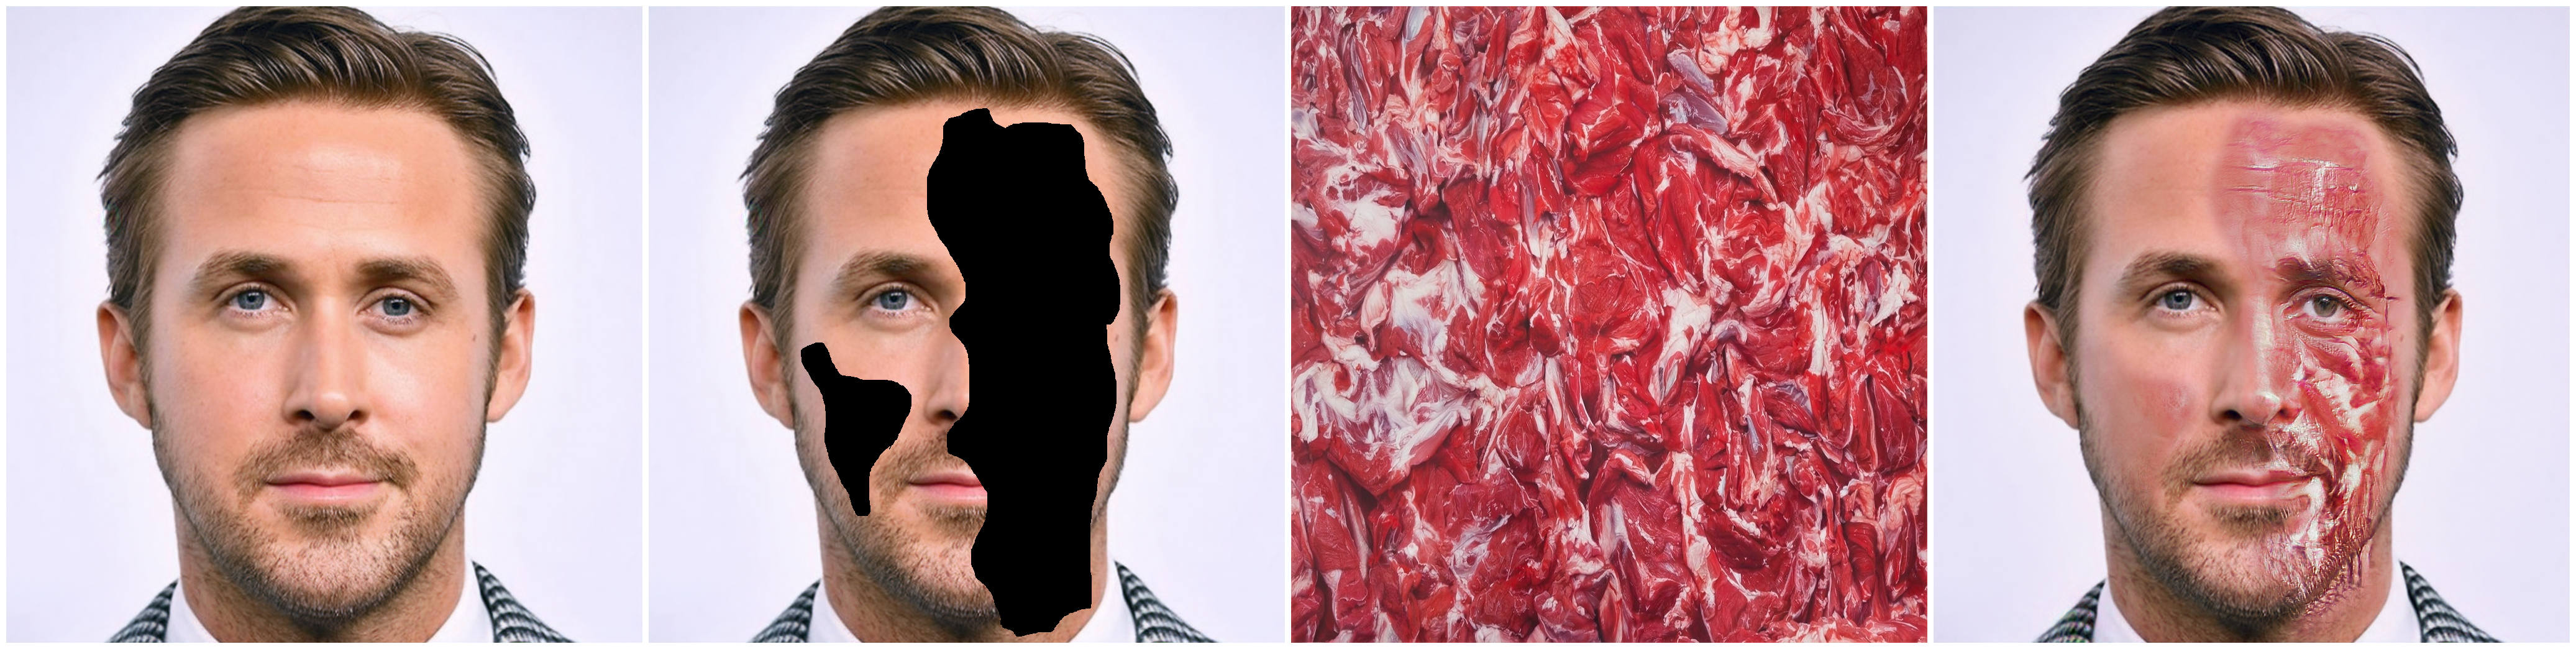
\includegraphics[width=0.95\linewidth]{images/style_ryan.jpg}
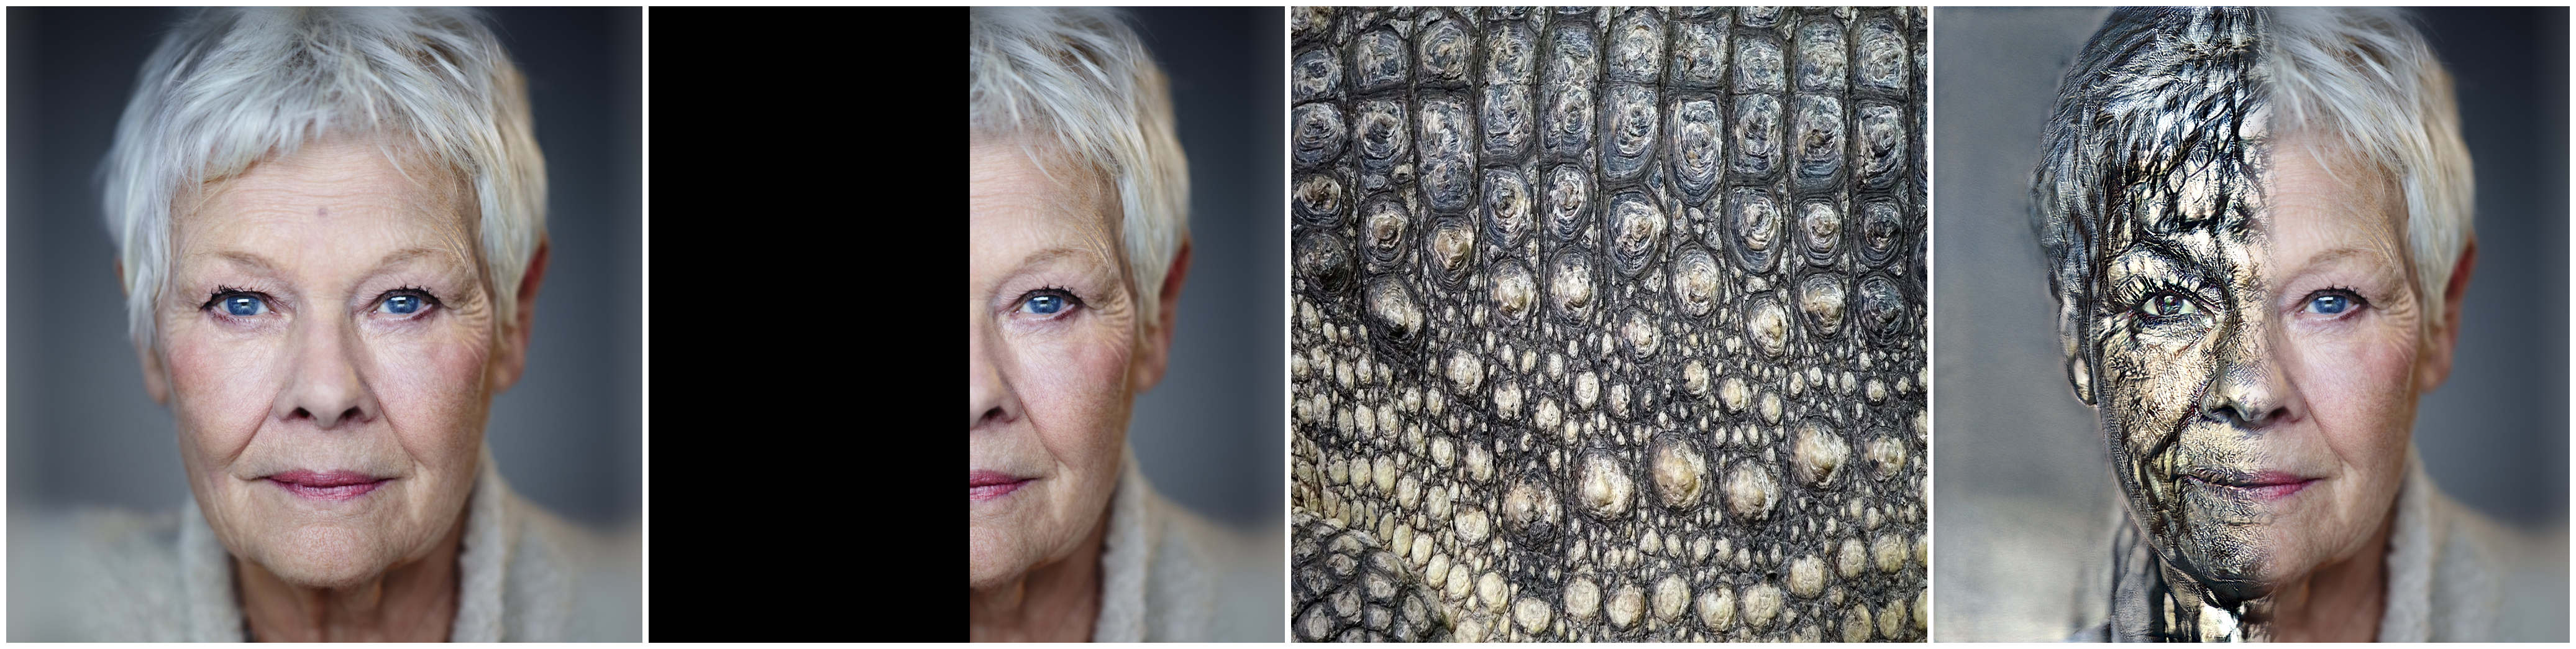
\includegraphics[width=0.95\linewidth]{images/style_judi.jpg}
\caption{\textbf{Illustration of local style transfer~\cite{abdal2020image2stylegan2}.} From left to right: base image, masked region, style image, local style transfer result.}
\label{fig:local_style_tranfer}
\end{figure}
}

\newcommand{\figinteractive}{
\begin{figure}[tbp]
\begin{center}
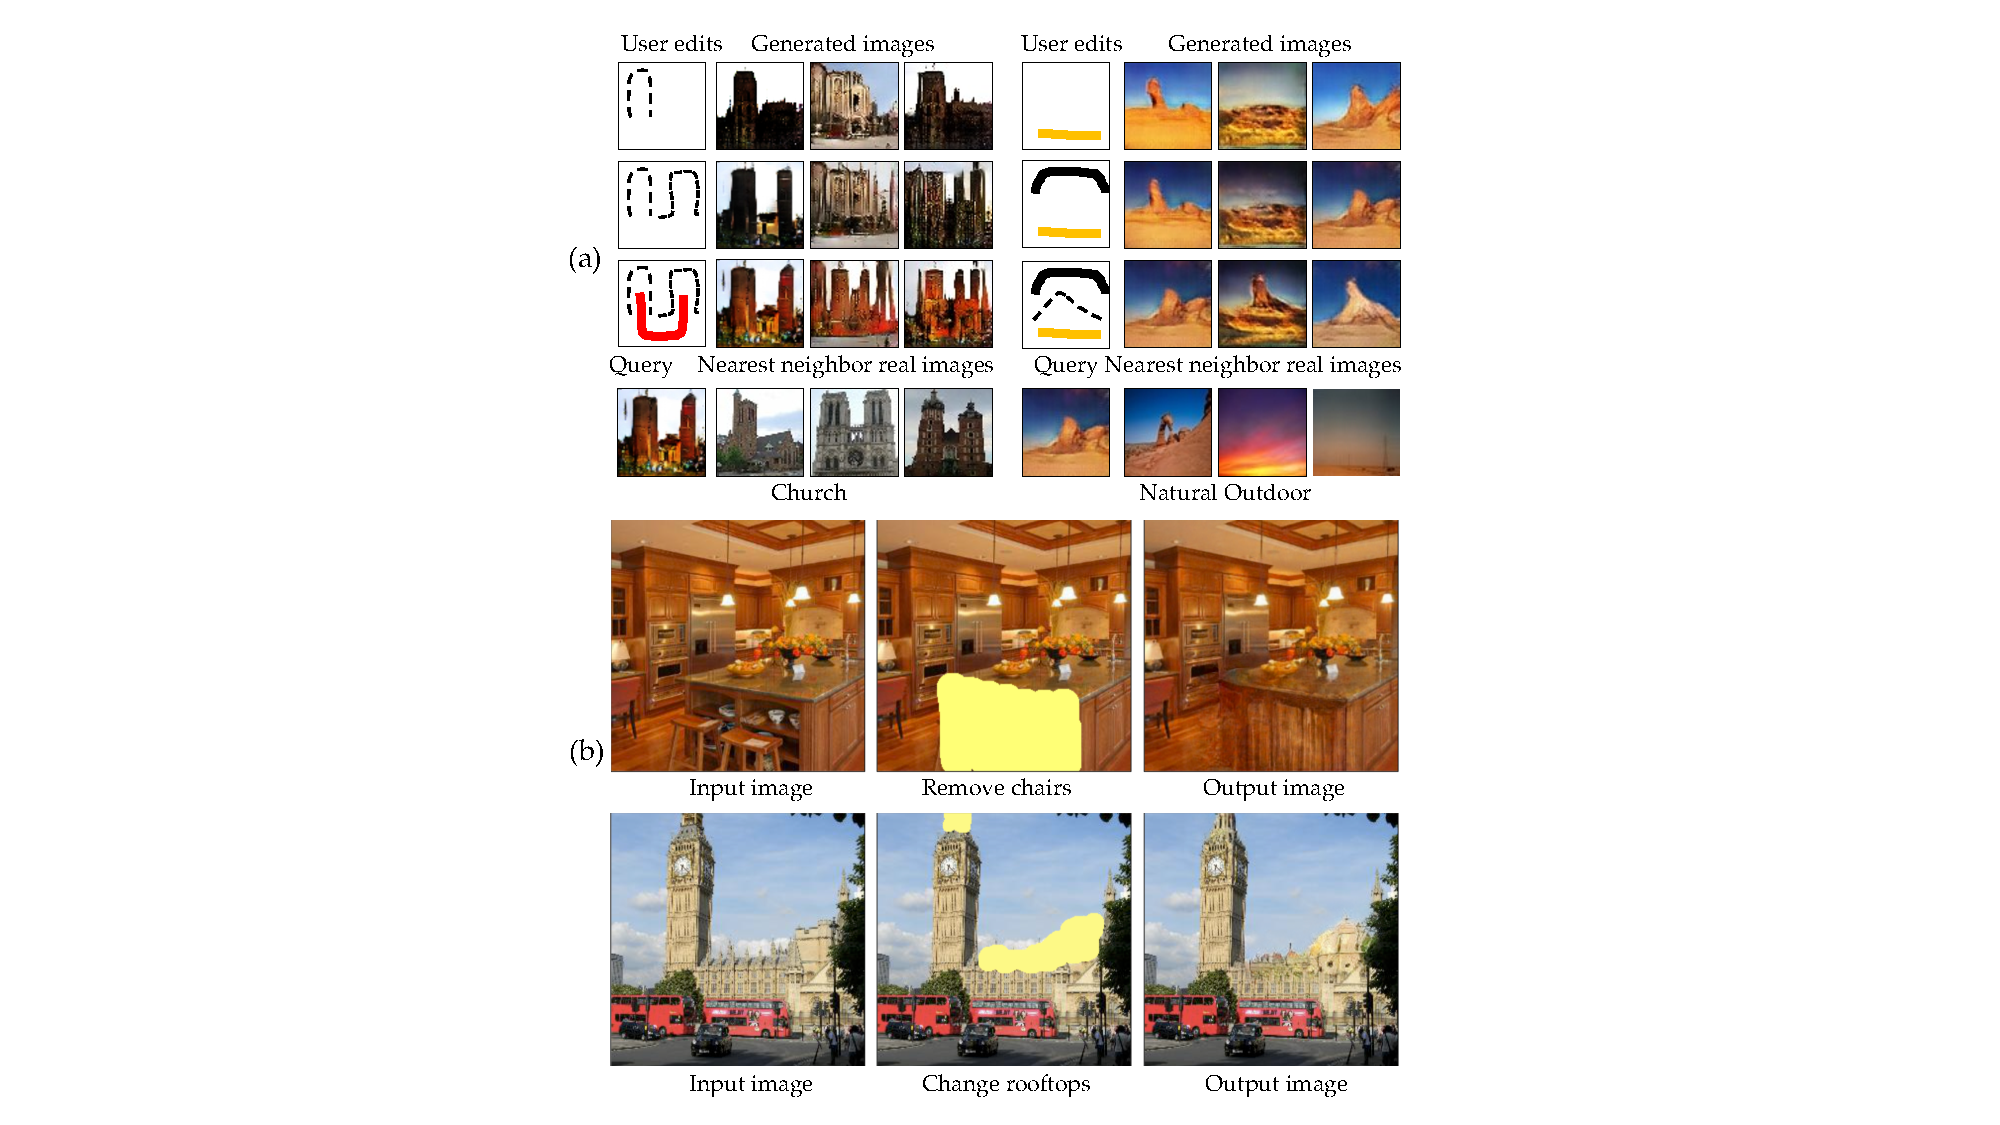
\includegraphics[width=0.95\linewidth]{images/interactive}
\end{center}
\caption{\textbf{Illustration of interactive image generation using GAN inversion.} (a) illustrates results from ~\cite{zhu2016generative}. The users are allowed to use the brush tools to generate an image from scratch and keep adding more scribbles or sketches for refinement. The last row shows the most similar real images to the generated images. Dashed line represents the sketch tool, and color scribble means the color brush.
(b) is from GANPaint~\cite{bau2019ganpaint}. The brushes can draw semantically meaningful units like removing chairs or adding rooftops.
}
\label{fig:interactive}
\end{figure}
}

\newcommand{\figdiffusion}{
\begin{figure}[tbp]
\begin{center}
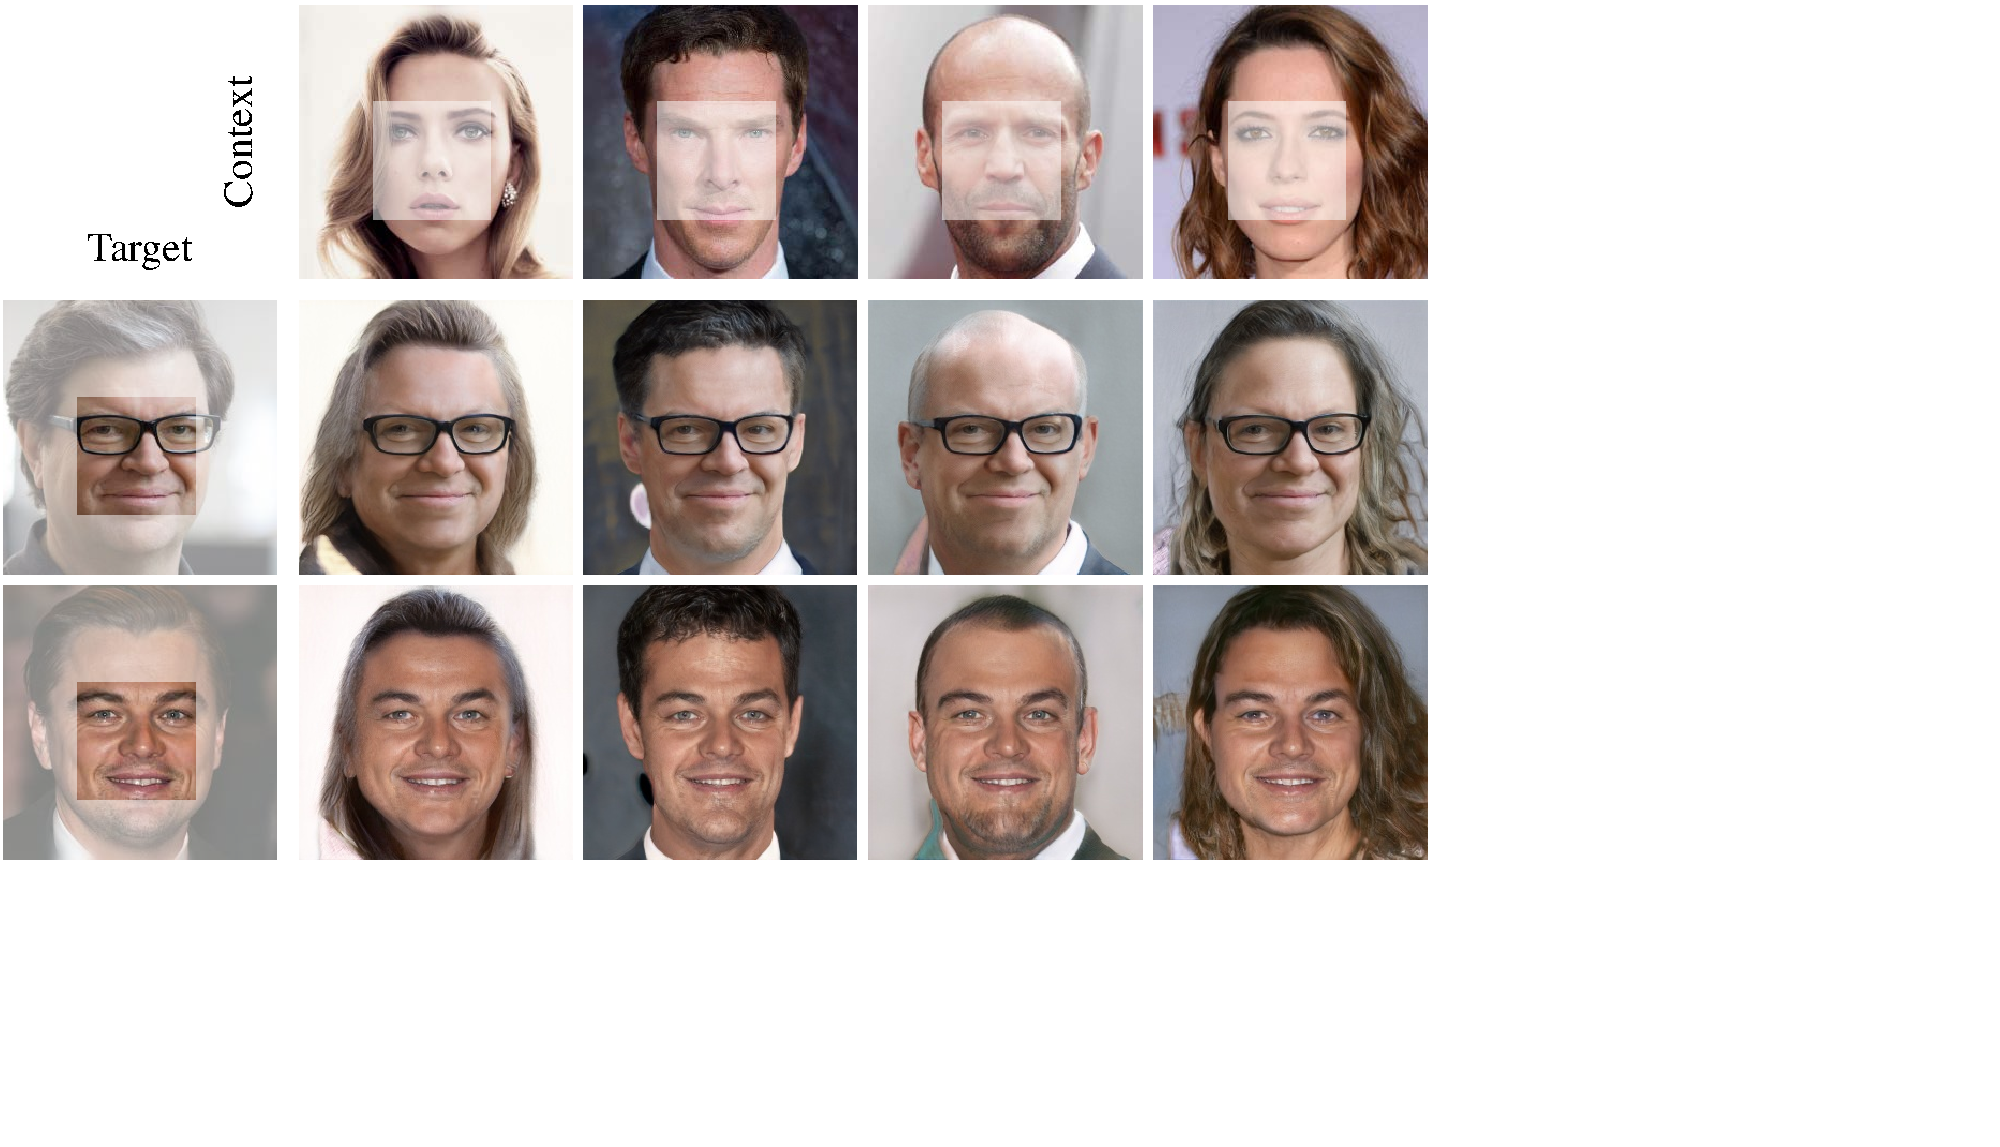
\includegraphics[width=0.95\linewidth]{images/diffusion.pdf}
\end{center}
\caption{\textbf{Semantic diffusion results using the in-domain GAN inversion method~\cite{zhu2020indomain}}. Target images in the first column are naturally diffused into context images in the first row with the identify preserved.}
\label{fig:diffusion}
\end{figure}
}

\newcommand{\tabfeature}{
\begin{table*}[htbp]
\caption{Characteristics of GAN inversion methods. `Type' includes Learning-based (L.), Optimization-based (O.), Hybrid (H.), and Closed-Form (C.) GAN inversion. I.-D., S.-A., L.-W., N.-I., R.-I. and O.-D. denote discovering the Interpretable Directions in a Supervised (S.) or an Unsupervised (U.) manner, Semantic-Aware, Layer-Wise, Non-Interference, Region-of-Interest, and Out-of-Distribution, respectively. GAN model and Dataset indicate which Pretrained Models are trained on which Dataset that a method is inverting, which can be found in Section~\ref{sec:model_data}.}
\label{tab:taxonomy}
\begin{center}
\scalebox{0.92}{
\begin{tabular}{c|c|c|c|c|c|c|c|c|c|c}
\toprule
Method  & Publication & Type &I.-D. &S.-A. &L.-W. &N.-I. &R.-I. &O.-D. &GAN Model & Dataset \\\hline
Zhu~\etal~\cite{zhu2016generative} &2016, NeurIPS &H. &\nxmark &\nxmark &\nxmark &\nxmark &\nxmark &\nxmark &\cite{radford2016dcgan} &\cite{yu2014local,zhou2014places,yu2015lsun}\\
Creswell~\etal~\cite{creswell2018inverting} &2018, TNNLS &O. &\nxmark &\nxmark &\nxmark &\nxmark &\nxmark &\nxmark &\cite{radford2016dcgan,gulrajani2017improved} &\cite{yu2014local,liu2015faceattributes}\\
GAN Dissection~\cite{bau2019gandissect} &2019, ICLR &O. &\nxmark &\ncmark &\ncmark &\nxmark &\ncmark &\nxmark &\cite{karras2017progressive} &\cite{yu2015lsun}\\
GAN Paint~\cite{bau2019ganpaint} & 2019, TOG &H. &\nxmark &\ncmark &\ncmark &\nxmark &\ncmark &\nxmark & \cite{karras2017progressive} & \cite{yu2015lsun}\\
Raj~\etal~\cite{raj2019gan} &2019, ICCV &O. &\nxmark &\nxmark &\nxmark &\nxmark &\nxmark &\nxmark &\cite{radford2016dcgan,zhang2019self} &\cite{yu2015lsun,lecun1998mnist,liu2015faceattributes}\\
GANSeeing~\cite{bau2019seeing} &2019, ICCV &H. &\nxmark &\ncmark &\ncmark &\nxmark & \nxmark &\nxmark &\cite{gulrajani2017improved,karras2017progressive,karras2019style}  &\cite{yu2015lsun}\\
Image2StyleGAN~\cite{abdal2019image2stylegan} &2019, ICCV &O. &\nxmark &\ncmark &\nxmark &\nxmark &\nxmark &\nxmark &\cite{karras2019style} &\cite{karras2019style} \\
Image2StyleGAN++~\cite{abdal2020image2stylegan2} &2020, CVPR &O. &\nxmark &\ncmark &\nxmark &\nxmark &\ncmark&\nxmark &\cite{karras2017progressive,karras2019style} &\cite{karras2017progressive,karras2019style}\\
mGANPrior~\cite{gu2020image} &2020, CVPR &O. &\nxmark &\ncmark &\ncmark &\ncmark &\nxmark &\ncmark &\cite{karras2017progressive,karras2019style} &\cite{karras2017progressive,karras2019style,yu2015lsun}\\
%IIN~\cite{esser2020invertible} &2020, CVPR &  &  &  &  &  &  &\\
Editing in Style~\cite{collins2020uncovering} &2020, CVPR &O. &\nxmark &\ncmark &\nxmark &\nxmark &\ncmark &\nxmark &\cite{karras2017progressive,karras2019style,karras2020analyzing} &\cite{karras2019style,yu2015lsun}\\
StyleRig~\cite{tewari2020stylerig} &2020, CVPR &L. &\nxmark &\ncmark &\nxmark &\nxmark &\nxmark &\nxmark &\cite{karras2019style} &\cite{karras2019style}\\
InterFaceGAN~\cite{shen2020interpreting} &2020, CVPR &L., O. &S. &\ncmark &\ncmark &\ncmark &\nxmark &\ncmark  &\cite{karras2017progressive,karras2019style} &\cite{karras2019style}\\
YLG~\cite{daras2020your} &2020, CVPR &O. &\nxmark &\nxmark &\nxmark &\nxmark &\nxmark &\ncmark &\cite{zhang2019self} &\cite{russakovsky2015imagenet}\\
GANRewriting~\cite{bau2020rewriting} &2020, ECCV &O. &\nxmark &\ncmark &\nxmark &\nxmark &\ncmark &\nxmark &\cite{karras2017progressive,karras2020analyzing} &\cite{yu2015lsun}\\
DGP~\cite{pan2020exploiting} &2020, ECCV &O. &\nxmark &\nxmark &\ncmark &\nxmark &\nxmark &\nxmark &\cite{brock2018large} &\cite{zhou2014places,russakovsky2015imagenet}\\
Huh~\etal~\cite{huh2020transforming} &2020, ECCV &O. &\nxmark &\ncmark &\nxmark &\nxmark &\ncmark &\ncmark &\cite{brock2018large,karras2020analyzing} &\cite{russakovsky2015imagenet,yu2015lsun,karras2019style}\\
IDInvert~\cite{zhu2020indomain} &2020, ECCV &H. &\nxmark &\ncmark &\nxmark &\nxmark &\nxmark &\ncmark &\cite{karras2019style}  &\cite{karras2019style,yu2015lsun}\\
StyleGAN2 Distillation~\cite{viazovetskyi2020distillation} &2020, ECCV &O. &S. &\ncmark &\nxmark &\ncmark &\nxmark &\ncmark &\cite{karras2020analyzing} &\cite{karras2019style}\\
GANSteering~\cite{jahanian2020steerability} &2020, ICLR &O. &S. &\ncmark &\nxmark &\nxmark &\nxmark &\nxmark &\cite{brock2018large,karras2019style,radford2016dcgan} &\cite{russakovsky2015imagenet,yu2015lsun,karras2019style}\\
GANLatentDiscovery~\cite{voynov2020latent} &2020, ICML &O. &U. &\ncmark &\nxmark &\nxmark &\nxmark &\nxmark &\cite{brock2018large,karras2017progressive} &\cite{karras2017progressive,jin2017towards,lecun1998mnist}\\
PIE~\cite{tewari2020pie} &2020, TOG &O. &S. &\ncmark &\nxmark &\ncmark &\nxmark &\ncmark &\cite{karras2019style}  &\cite{karras2019style}\\
StyleFlow~\cite{abdal2020styleflow} &2020, arxiv &O. &S. &\ncmark &\nxmark &\ncmark &\nxmark &\ncmark &\cite{karras2019style,karras2020analyzing}  &\cite{karras2019style,yu2015lsun}\\
GANSpace~\cite{eric2020GANSpace} &2020, arxiv &O. &U. &\ncmark &\ncmark &\ncmark &\nxmark &\nxmark &\cite{brock2018large,karras2019style,karras2020analyzing} &\cite{karras2017progressive,yu2015lsun}\\
Nitzan~\etal~\cite{nitzan2020harness} &2020, arxiv &L. &\nxmark &\ncmark &\nxmark &\ncmark &\nxmark &\nxmark &\cite{karras2019style}  &\cite{karras2017progressive,karras2019style}\\
% Li~\etal~\cite{li2020latent} &2020, arxiv &O. &\nxmark &\ncmark &\nxmark &\ncmark &\nxmark &\nxmark &\cite{gulrajani2017improved}  &\cite{xiao2017fashion,yu2017jittor}\\
SeFa~\cite{shen2020closedform} &2020, arxiv &C. &U. &\ncmark &\ncmark &\ncmark &\ncmark &\ncmark &\cite{karras2017progressive,brock2018large,karras2019style,karras2020analyzing} &\cite{naik2014streetscore,karras2017progressive,karras2019style,yu2015lsun,russakovsky2015imagenet}\\
Aberdam~\etal~\cite{aberdam2020invert} &2020, arxiv &O. &\nxmark &\nxmark &\ncmark &\nxmark &\nxmark &\nxmark & a two-layer model & \cite{lecun1998mnist} \\
StyleGAN-Encoder~\cite{guan2020faster} &2020, arxiv &L. &\nxmark &\ncmark &\nxmark &\ncmark &\nxmark &\nxmark &\cite{karras2019style} &\cite{karras2017progressive,karras2019style,chen2014cross}\\
GH-Feat~\cite{xu2020ghfeat} &2020, arxiv &L. &\nxmark &\ncmark &\ncmark &\nxmark &\nxmark &\nxmark &\cite{karras2019style} &\cite{lecun1998mnist,yu2015lsun,karras2019style}\\
pSp~\cite{richardson2020encoding} &2020, arxiv &L. &\nxmark &\ncmark &\ncmark &\ncmark &\ncmark &\ncmark &\cite{karras2020analyzing} &\cite{karras2017progressive}\\
Style Intervention~\cite{liu2020style} &2020, arxiv &O. &S. &\ncmark &\nxmark &\ncmark &\ncmark &\ncmark &\cite{karras2020analyzing} &\cite{liu2020style}\\
StyleSpace~\cite{wu2020stylespace} &2020, arxiv &O.&S. &\ncmark &\nxmark &\ncmark &\ncmark &\ncmark &\cite{karras2020analyzing} &\cite{karras2019style,yu2015lsun}\\
Lu~\etal~\cite{lu2020discovery} &2020, arxiv &L. &U. &\ncmark &\nxmark &\ncmark &\nxmark &\nxmark &\cite{karras2020analyzing,karras2017progressive,miyato2018spectral} &\cite{karras2019style,russakovsky2015imagenet}\\
Cherepkov~\etal~\cite{cherepkov2020navigating} &2020, arxiv &O. &U. &\ncmark &\nxmark &\ncmark &\nxmark &\ncmark &\cite{karras2020analyzing} &\cite{karras2019style,yu2015lsun}\\
Nurit~\etal~\cite{nurit2020steerability} &2020, arxiv &C. &U. &\ncmark &\nxmark &\ncmark &\nxmark &\nxmark &\cite{brock2018large} &\cite{russakovsky2015imagenet} \\

\bottomrule
\end{tabular}
}
\end{center}
\end{table*}
% \footnotetext[1]{They use a self-defined two-layer GAN model.}
}